% Drawing 154/06-8 -- folder 154, batch 06, archive page 111 (PDF page 112).
% Transcription: dessins en couleur : deux droites vert clair $D$ et $\overline{D}$ qui se croisent en un point multiple d'un faisceau de droites orange, de part et d'autre d'une droite brune horizontale, avec deux flèches courbes qui indiquent le passage de l'une à l'autre ; sur les droites orange, de chaque côté, des points marqués $u$, $v$, $w$, $u'$, $v'$, $w'$ et leurs barrés $\bar{u}$, $\bar{v}$, $\bar{w}$, $\bar{u}'$, \ldots, au milieu $r$, $s$, $t$, $\bar{r}$, $\bar{s}$, $\bar{t}$, à droite $a$, $a'$, $\bar{a}$, $\bar{a}'$ et $x$, $y$, $z$, $x'$, $y'$, $z'$ avec leurs barrés ; en bas à gauche une étiquette « $\overline{D}{}^{\ast}$ » (\uncertain{lue}). Au-dessus, une première version du même dessin, moins complète. Plus bas, un croisement de droites orange enjambé par une courbe vert clair en tirets, avec des flèches et deux arcs (noir et bleu) marqués ; à droite, deux petits faisceaux orange sur une droite vert clair
% Kind: lines D and D-bar crossing at a multiple point; first version; crossing with a dashed generisation; two small pencils. Method 2 (schematic redraw from the facsimile). Status: partial.
% Notes: Over a typed notice (upside down; not reproduced). Two light green lines D and D-bar crossing at a multiple point of a pencil of orange lines, on either side of a horizontal brown line, with curved arrows for the passage from one to the other; on the orange lines on each side points marked u, v, w, u', v', w' and their barred versions, r, s, t in the middle, a, a', x, y, z, x', y', z' on the right (these point labels are not reproduced individually; only D, D-bar, D-bar* are placed); above it a first, less complete version of the same drawing. Lower, a crossing of orange lines straddled by a dashed light green curve, with arrows and two marked arcs (black and blue); to the right two small orange pencils on a light green line. Read from the page view.
% Coordinates: 1 unit = 1 mm = 1/100 of the crop width (bbox in page fractions: [0.121, 0.098, 0.501, 0.47]).
% Redrawn by Claude (claude-opus-5-5), issue #73, 2026-11-07; not checked by a human; not compiled (no TeX in the session).
% Rights: reproduces part of the work -- behind RENDER_TRANSCRIPTS, never published by itself.
\documentclass[tikz,border=3pt]{standalone}
\usepackage{amsmath,amssymb}
\usetikzlibrary{patterns,arrows.meta}
\tikzset{Or/.style={orange!90!black}, Ye/.style={yellow!80!orange}, Lg/.style={green!60!black!70}, Dg/.style={green!45!black}, Br/.style={brown!80!black}, Rd/.style={red!85!black}, Bl/.style={blue!70!black}, Gy/.style={black!40}, pencil/.style={black!45}, struck/.style={black!35}, mark/.style={circle,draw,inner sep=1.3pt}, pt/.style={circle,fill,inner sep=0.9pt}, opt/.style={circle,draw,fill=white,inner sep=1.1pt}}
\begin{document}
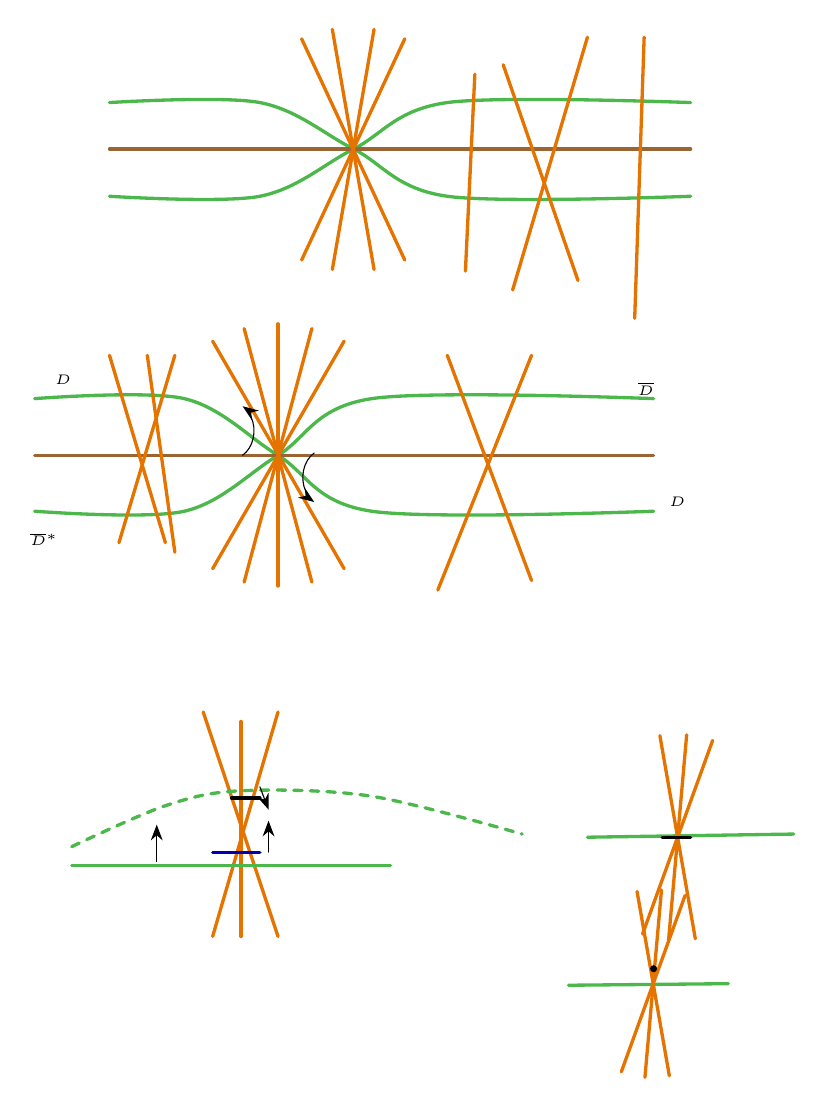
\begin{tikzpicture}[x=1mm,y=1mm,line cap=round,line join=round,font=\scriptsize]
\draw[Lg,very thick] plot[smooth, tension=0.55] coordinates {(11.9,-13.1) (31,-13.1) (42.9,-19) (54.8,-25) (85.7,-25)};
\draw[Lg,very thick] plot[smooth, tension=0.55] coordinates {(11.9,-25) (31,-25) (42.9,-19) (54.8,-13.1) (85.7,-13.1)};
\draw[Br,very thick] (11.9,-19) -- (85.7,-19);
\draw[Or,very thick] (36.3,-33.1) -- (49.4,-5);
\draw[Or,very thick] (40.2,-34.3) -- (45.5,-3.8);
\draw[Or,very thick] (45.5,-34.3) -- (40.2,-3.8);
\draw[Or,very thick] (49.4,-33.1) -- (36.3,-5);
\draw[Or,very thick] (61.9,-8.3) -- (71.4,-35.7);
\draw[Or,very thick] (72.6,-4.8) -- (63.1,-36.9);
\draw[Or,very thick] (58.3,-9.5) -- (57.1,-34.5);
\draw[Or,very thick] (79.8,-4.8) -- (78.6,-40.5);
\draw[Lg,very thick] plot[smooth, tension=0.55] coordinates {(2.4,-50.7) (21.4,-50.7) (33.3,-57.9) (45.2,-65) (81,-65)};
\draw[Lg,very thick] plot[smooth, tension=0.55] coordinates {(2.4,-65) (21.4,-65) (33.3,-57.9) (45.2,-50.7) (81,-50.7)};
\draw[Br,very thick] (2.4,-57.9) -- (81,-57.9);
\draw[Or,very thick] (25,-72.3) -- (41.7,-43.4);
\draw[Or,very thick] (29,-74) -- (37.6,-41.8);
\draw[Or,very thick] (33.3,-74.5) -- (33.3,-41.2);
\draw[Or,very thick] (37.6,-74) -- (29,-41.8);
\draw[Or,very thick] (41.7,-72.3) -- (25,-43.4);
\draw[Or,very thick] (11.9,-45.2) -- (19,-69);
\draw[Or,very thick] (20.2,-45.2) -- (13.1,-69);
\draw[Or,very thick] (16.7,-45.2) -- (20.2,-70.2);
\draw[Or,very thick] (54.8,-45.2) -- (65.5,-73.8);
\draw[Or,very thick] (65.5,-45.2) -- (53.6,-75);
\draw[-{Stealth[length=2mm]}] (37.9,-57.6) arc[start angle=120, end angle=240, x radius=2.9, y radius=3.6];
\draw[-{Stealth[length=2mm]}] (28.8,-57.9) arc[start angle=-60, end angle=60, x radius=2.9, y radius=3.6];
\node[inner sep=1pt] at (6,-48.3) {\tiny $D$};
\node[inner sep=1pt] at (80,-49.5) {\tiny $\overline{D}$};
\node[inner sep=1pt] at (84,-63.8) {\tiny $D$};
\node[inner sep=1pt] at (3.6,-68.6) {\tiny $\overline{D}{}^{\ast}$};
\draw[Or,very thick] (23.8,-90.5) -- (33.3,-119);
\draw[Or,very thick] (33.3,-90.5) -- (25,-119);
\draw[Or,very thick] (28.6,-91.7) -- (28.6,-119);
\draw[Lg,very thick] (7.1,-110) -- (47.6,-110);
\draw[Lg,dashed,very thick] plot[smooth, tension=0.55] coordinates {(7.1,-107.6) (19,-102.4) (28.6,-100.5) (45.2,-101.2) (64.3,-106)};
\draw[very thick] (27.4,-101.4) -- (31,-101.4);
\draw[Bl,very thick] (25,-108.3) -- (31,-108.3);
\draw[-{Stealth[length=2mm]}] (17.9,-109.5) -- (17.9,-104.8);
\draw[-{Stealth[length=2mm]}] (32.1,-108.3) -- (32.1,-104.3);
\draw[-{Stealth[length=2mm]}] (31,-100) -- (32.1,-102.9);
\draw[Lg,very thick] (72.6,-106.4) -- (98.8,-106);
\draw[Or,very thick] (79.6,-118.7) -- (88.5,-94.1);
\draw[Or,very thick] (82.9,-119.5) -- (85.2,-93.4);
\draw[Or,very thick] (86.3,-119.3) -- (81.8,-93.5);
\draw[very thick] (82.1,-106.4) -- (85.7,-106.4);
\draw[Lg,very thick] (70.2,-125.2) -- (90.5,-125);
\draw[Or,very thick] (76.9,-136.2) -- (85,-113.8);
\draw[Or,very thick] (79.9,-136.9) -- (82,-113.1);
\draw[Or,very thick] (83,-136.7) -- (78.9,-113.3);
\node[pt] at (81,-123.1) {};
\end{tikzpicture}
\end{document}
